\documentclass[a4paper]{article}

\usepackage[english]{babel}
\usepackage[utf8]{inputenc} 
\usepackage{amsmath,amssymb}
\usepackage{parskip} 
\usepackage[usenames,dvipsnames,table]{xcolor} 
\usepackage{fancyvrb} 
\PassOptionsToPackage{hyphens}{url}\usepackage{hyperref} 
\DeclareMathOperator{\E}{\mathbb{E}}
\usepackage{amsthm}
\newtheorem{theorem}{Theorem}
\usepackage{mdframed}
\usepackage{xcolor}
\usepackage{framed}
\usepackage{listings}
\usepackage{graphicx} % Allows including images
\usepackage{booktabs} % Allows the use of \toprule, \midrule and \bottomrule in tables
\usepackage{amsmath,amssymb}
\usepackage{tikz}
\usetikzlibrary{arrows}
\usepackage{mathtools}
\usepackage{float}
\usepackage{fancyvrb} 
\usepackage{pgfplots}
\pgfplotsset{compat=newest}
%% the following commands are needed for some matlab2tikz features
\usetikzlibrary{plotmarks}
\usetikzlibrary{arrows.meta}
\usepgfplotslibrary{patchplots}
\usepackage{grffile}
\usepackage{amsmath}
\usetikzlibrary{patterns}
\usepackage{subcaption}
\usepackage{rotating}
\usepackage{lscape}
\usepackage{standalone}
\usepackage{enumitem}
\usepackage{shadethm}
\usepackage{setspace}
\usetikzlibrary{positioning}

\newshadetheorem{thm}{Theorem}
\definecolor{shadethmcolor}{HTML}{EDF8FF}
\definecolor{shaderulecolor}{HTML}{45CFFF}
\setlength{\shadeboxrule}{.4pt}
\setlength{\parindent}{5ex}

\makeatletter
\@addtoreset{equation}{section}
\@addtoreset{equation}{subsection}
\@addtoreset{equation}{subsubsection}
\@addtoreset{equation}{paragraph}
\@addtoreset{equation}{subparagraph}
\makeatother


\hypersetup{
	colorlinks = true,
	urlcolor   = blue,
	linkcolor  = blue,
	citecolor  = red
}

\usepackage{logicproof} 
\usepackage{tikz} 
\usetikzlibrary{trees,positioning}
\usepackage{tikz}


\DeclareMathOperator{\di}{d\!}
\newcommand*\Eval[3]{\left.#1\right\rvert_{#2}^{#3}}


% ------------------------------------------------------------------------------------
% ------------------------------------------------------------------------------------





\title{\large Problem Set V}
\author{\small ECO 7427 - Econometric Theory II \\
	\small{}}
\date{\small{\textit{  \textbf{{\color{blue} \href{https://github.com/armandkapllani}{Armand Kapllani} \\ University of Florida Economics}}} \\ Spring 2018}}


\begin{document}
	\maketitle

		\pagestyle{empty}
		
		\def\layersep{2.5cm}
		
\section*{Social Networks}

Let $N = \Big\{ 1, 2, 3, 4, 5, 6 \Big\}$ and consider the following network $(N, g)$. 
\vspace{2cm}


\tikzset{main node/.style={circle,fill=blue!30,draw,minimum size=1cm,inner sep=0pt},}
				
\begin{figure}[ht!]
	\caption{Undirected and Unweighted Network} \label{fig:M1}		
\begin{tikzpicture}
	
	% Construct the vertices
	\node[main node](1){$1$};
	\node[main node](2) [below right = 3cm and 3cm of 1] {$2$};
	\node[main node](3) [below = 5cm  of 1] {$3$};
	\node[main node](6) [left = 3cm of 1] {$6$};
	\node[main node](4) [below = 5cm  of 6] {$4$};
	\node[main node](5) [left = 10 cm of 2] {$5$};

	% Link the vertices through edges 
	\path[draw,thick]
	(1) edge  [red] node {} (2)
	(2) edge [red] node {} (3)
	(3) edge [red] node {} (1)
	(4) edge [red] node {} (3)
	(5) edge [red] node {} (3)
	(6) edge [red] node {} (3)
	(4) edge [red] node {} (6)
	(4) edge [red] node {} (1);

\end{tikzpicture}
\end{figure}		

\vspace{5cm}

\noindent \textbf{{\color{blue}  Construct the adjacency matrix}}: 

\[ g = 
\begin{bmatrix}
0 & 1 & 1 & 1 & 0 & 0 \\
1 & 0 & 1 & 0 & 0 & 0 \\
1 & 1 & 0 & 1 & 1 & 1 \\
1 & 0 & 1 & 0 & 0 & 1 \\
0 & 0 & 1 & 0 & 0 & 0 \\
0 & 0 & 1 & 1 & 0 & 0 \\
\end{bmatrix}
\]

\noindent To compute the degree of each vertex we sum across each row  

\begin{equation}
	d_i(g) = \sum_{j} g_{ij}
\end{equation}

\noindent \textbf{{\color{blue} The neighborhood of each vertex}}: 

\begin{table}[ht!]
	\centering
	\captionof{table}{Neighborhood of each vertex} \label{tab:title} 
	\begin{tabular}{l@{\hskip 0.5in}l}
		Vertex & $N_i(g)$\\
		\hline\hline
		
		N = 1 &  $\big\{ 2, 3, 4 \big\}$ \\
		N = 2 & $\big\{  1, 3 \big\}$ \\
		N = 3 & $\big\{  1, 2, 4, 5, 6 \big\}$ \\
		N = 4 & $\big\{ 1, 3, 6 \big\}$ \\
		N = 5 & $\big\{  3 \big\}$ \\
		N = 6 & $\big\{  3, 4 \big\}$ \\
		
		\bottomrule[1pt]
	\end{tabular}
\end{table}



\noindent \textbf{{\color{blue} The degree of each node}}: 

\begin{table}[ht!]
	\centering
	\captionof{table}{Degree of each vertex in the network} \label{tab:title} 
	\begin{tabular}{l@{\hskip 0.5in}c}
		Vertex & Degree\\
		\hline\hline

		N = 1 & 3 \\
		N = 2 & 2 \\
		N = 3 & 5 \\
		N = 4 & 3\\
		N = 5 & 1 \\
		N = 6 & 2 \\
		
		\bottomrule[1pt]
	\end{tabular}
\end{table}


\begin{figure}[ht!]
	\centering
		\captionof{figure}{Degree Histogram} \label{tab:figure}
		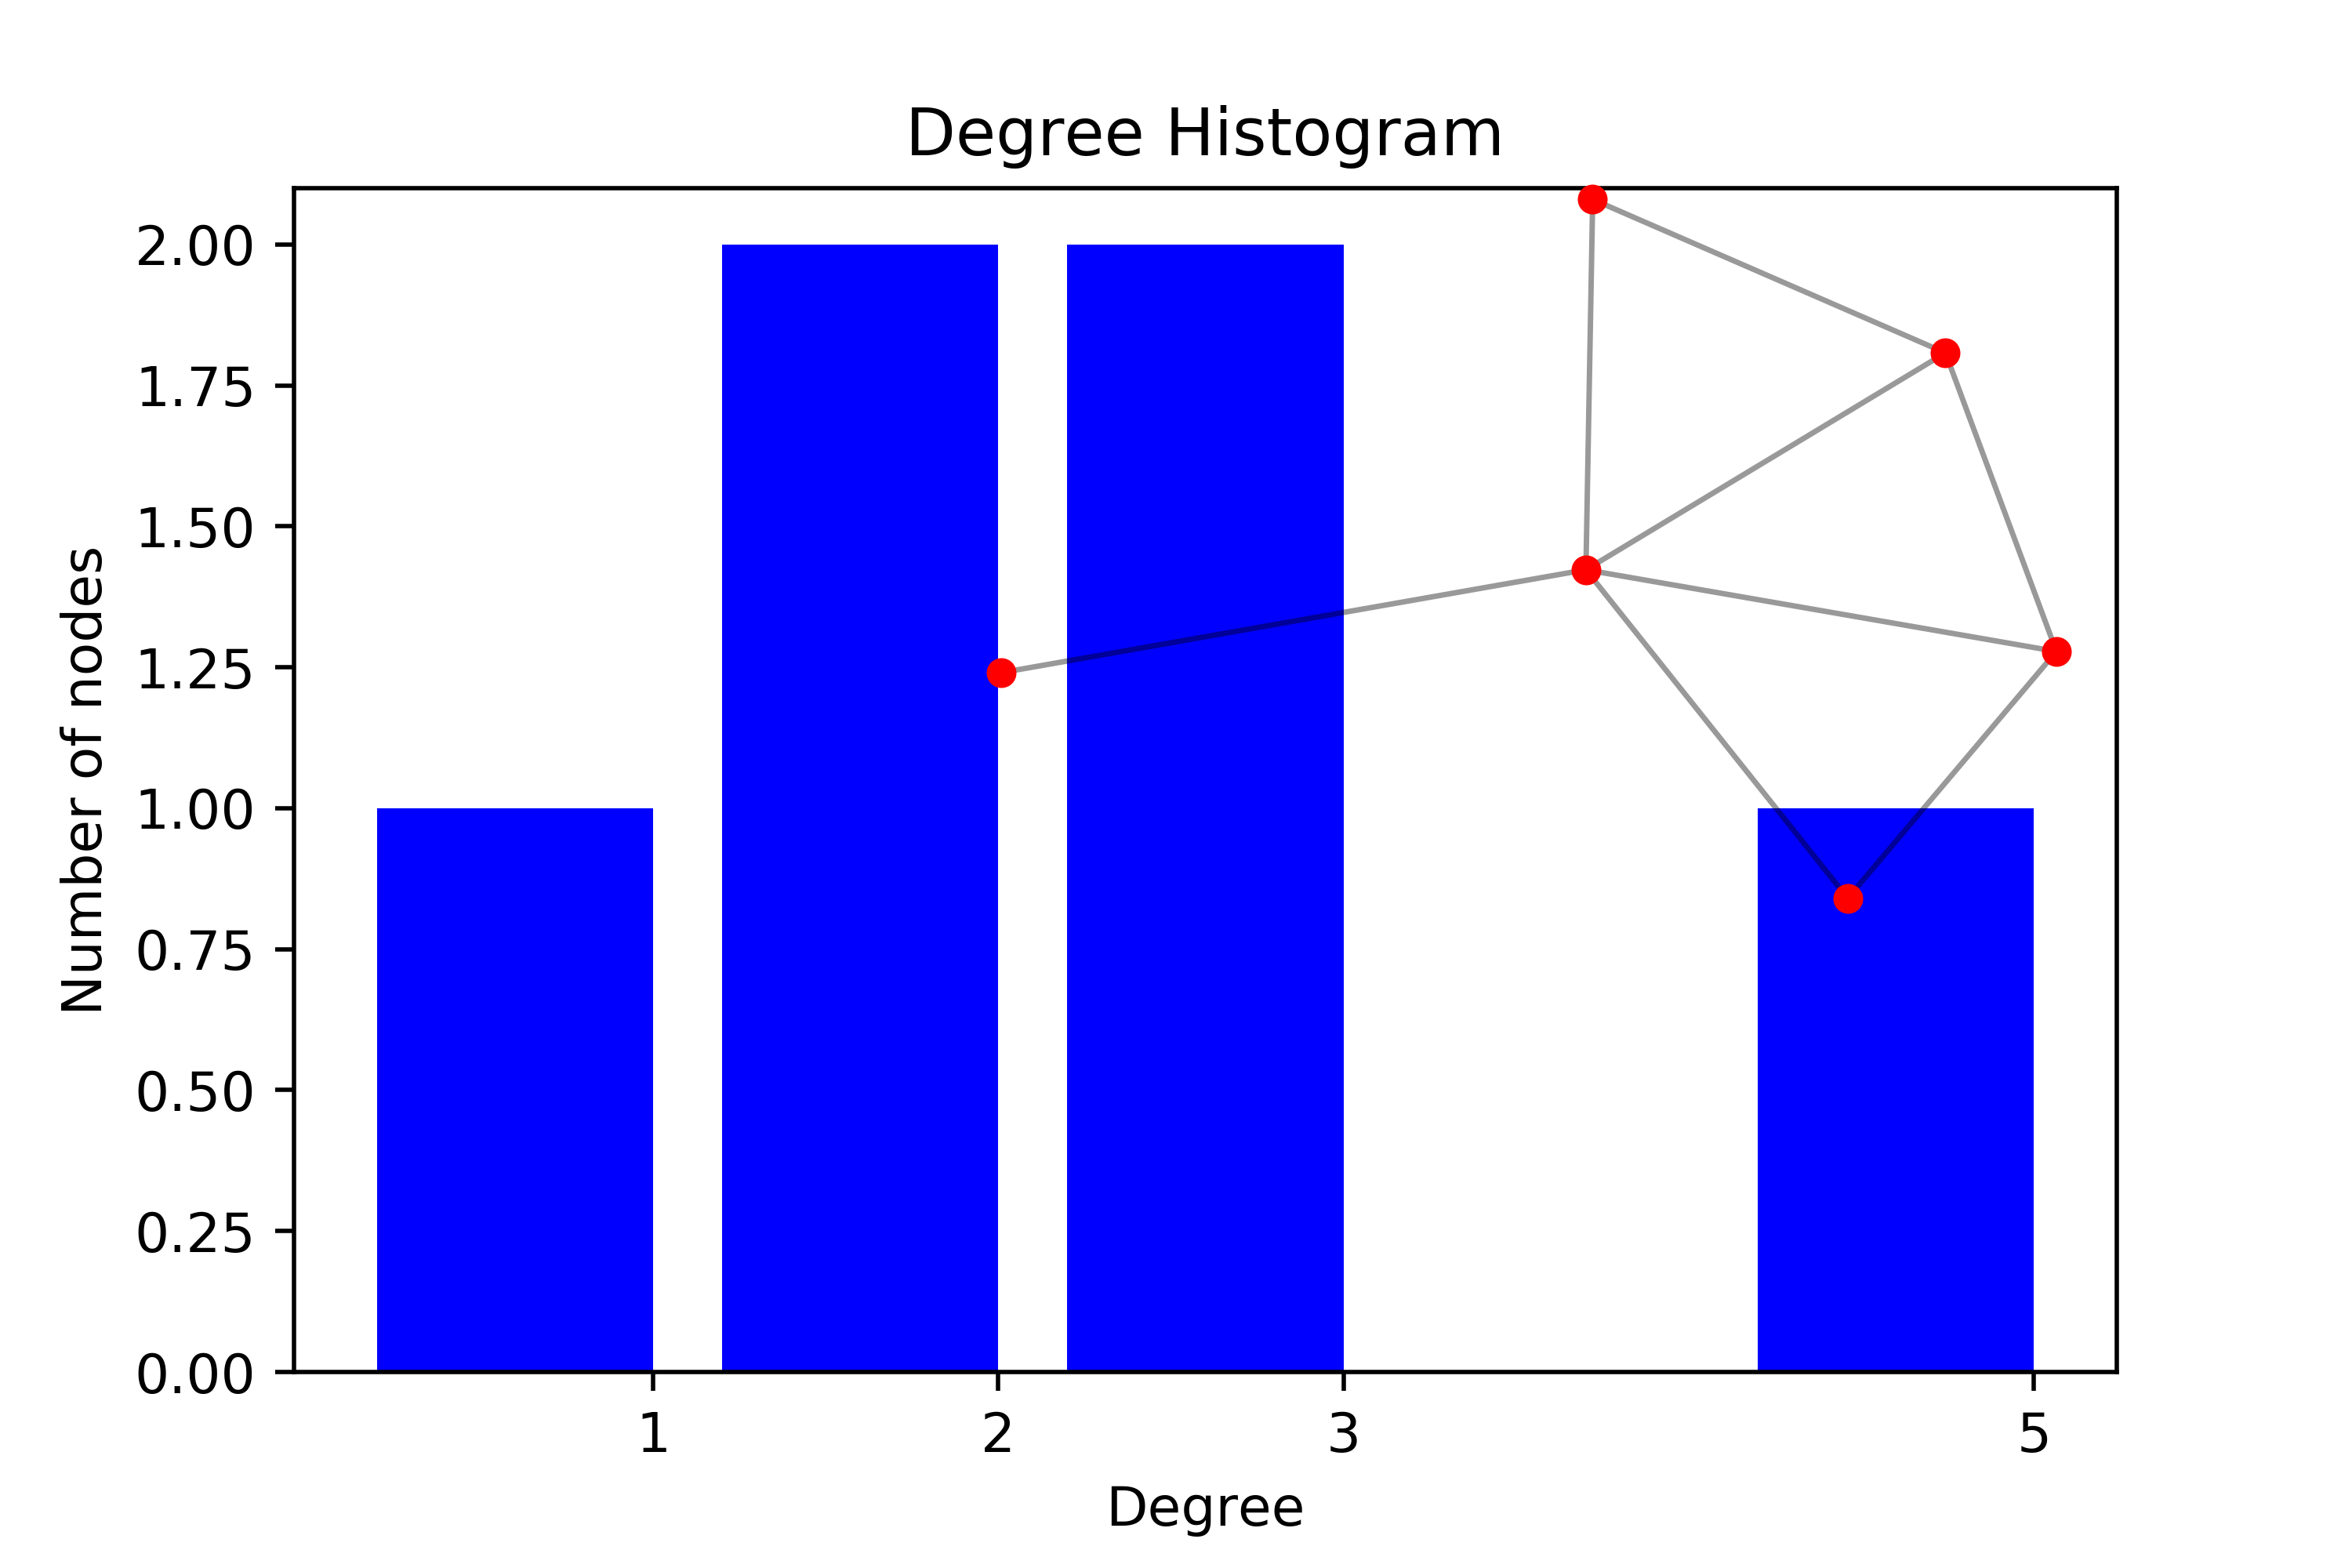
\includegraphics[scale=0.9]{degree_histogram.png}
\end{figure}



\noindent \textbf{{\color{blue} Average degree of the network $g \in G(N)$}}: 

\begin{equation}
	\frac{1}{N} \sum_{i\in N} d_i(g) = \frac{1}{6} \big[ 3 + 2 + 5 + 3 + 1 + 2 \big] = \frac{8}{3}
\end{equation}

\noindent \textbf{{\color{blue} The density of the network $g \in G(N)$}}:

\begin{equation}
	\frac{\sum_{i\in N} d_i(g)}{n(n-1)} = \frac{ \frac{1}{n} \sum_{i\in N} d_i(g) }{n-1} = \frac{8/3}{5} = \frac{8}{15}
\end{equation}

\noindent \textbf{{\color{blue} The individual clustering of the six vertices}}: 

\begin{equation}
	CI_i(g) = \frac{\Big\{ jk\in g | k \ne j, j\in N_i(g), k\in N_i(g) \Big\}}{d_i(g)\big[ d_i(g)-1\big] }
\end{equation}

\begin{table}[ht!]
	\centering
	\captionof{table}{Individual clustering of each vertex} \label{tab:title} 
	\begin{tabular}{l@{\hskip 0.5in}c}
		Vertex & $CI_i(g)$\\
		\hline\hline
		
		N = 1 & 2/3  \\
		N = 2 &  1 \\
		N = 3 &  3/10 \\
		N = 4 & 2/3 \\
		N = 5 & 0 \\
		N = 6 & 1 \\
		
		\bottomrule[1pt]
	\end{tabular}
\end{table}

\noindent \textbf{{\color{blue} The average clustering coefficient}}:

\begin{equation}
CI^{\text{Avg}}(g)=\frac{1}{n}\sum_{i\in N}CI_i(g) = \frac{1}{6} \big[ \frac{2}{3} + 1 + \frac{3}{10} + \frac{2}{3} + 0 + 1 \big] = \frac{109}{180}
\end{equation} 

\vspace{1cm}

\noindent \textbf{{\color{blue} Degree centrality for each vertex}}:

\begin{equation}
CI_i(g) = \frac{\Big\{ jk\in g | k \ne j, j\in N_i(g), k\in N_i(g) \Big\}}{d_i(g)\big[ d_i(g)-1\big] }
\end{equation}

\begin{table}[ht!]
	\centering
	\captionof{table}{Degree centrality for each vertex} \label{tab:title} 
	\begin{tabular}{l@{\hskip 0.5in}c}
		Vertex & $CI_i(g)$\\
		\hline\hline
		
		N = 1 & 3/5  \\
		N = 2 & 2/5 \\
		N = 3 & 1\\
		N = 4 &  3/5 \\
		N = 5 &  1/5 \\
		N = 6 &  2/5 \\
		
		\bottomrule[1pt]
	\end{tabular}
\end{table}

Hence from Table $4$ we can see that vertex $3$ is well connected in terms of direct connections as it has the highest degree of centrality. However using this measure alone we cannot tell if vertex $3$ is well located in the network $(N, g)$. 

\noindent \textbf{{\color{blue} Closeness centrality fo each vertex}}:

\begin{equation}
	C_{i}(g) = \frac{1}{\frac{1}{n-1}\sum_{j\ne i}l(i,j)}
\end{equation}

where $l(i,j)$ denotes the number of links in the \textbf{shortest path} between $i$ and $j$. 

\begin{table}[ht!]
	\centering
	\captionof{table}{Closeness centrality fo each vertex} \label{tab:title} 
	\begin{tabular}{l@{\hskip 0.5in}c}
		Vertex & $C_i (g)$\\
		\hline\hline
		
		N = 1    &   5/7 \\
		N = 2   &  5/8 \\
		N = 3   &  1    \\
		N = 4   &  5/7 \\
		N = 5   &  5/9 \\
		N = 6   &  5/8 \\
		
		\bottomrule[1pt]
	\end{tabular}
\end{table}


\noindent \textbf{{\color{blue} Decay centrality for each vertex}}:

\begin{equation}
	D_i^(g) = \sum_{j\ne i}\delta^{l(i,j)}
\end{equation}

where $l(i,j)$ denotes the number of links in the \textbf{shortest path} between $i$ and $j$. 

\begin{table}[ht!]
	\centering
	\captionof{table}{Decay centrality fo each vertex} \label{tab:title} 
	\begin{tabular}{l@{\hskip 0.5in}c@{\hskip 0.5in}c}
		Vertex & $D^\delta_i (g)$  & $\delta = 1/2$ \\
		\hline\hline
		
		N = 1    &  $\delta(3+2\delta)$ & 2 \\
		N = 2   &  $\delta(2+3\delta)$ & 7/4 \\
		N = 3   &  $5\delta$ &  5/2 \\
		N = 4   &  $\delta(3+2\delta)$ & 2\\
		N = 5   &  $\delta(1+4\delta)$ & 3/2 \\
		N = 6   &  $\delta(2+3\delta)$ & 7/4\\
		
		\bottomrule[1pt]
	\end{tabular}
\end{table}

\vspace{6cm}
\noindent \textbf{{\color{blue} Betweenness centrality for each vertex}}:

\begin{equation}
	Ce_i^B(g) = \sum_{k\ne j: i \not\in \{ k, j \}} \frac{P_i(kj)/P(kj)}{\frac{1}{2}(n-1)(n-2)}
\end{equation}

\begin{table}[ht!]
	\centering
	\captionof{table}{Betweenness centrality of a vertex} \label{tab:title} 
	\begin{tabular}{l@{\hskip 0.5in}c@{\hskip 0.5in}c}
		Vertex & $P_i(k,j)$ &$Ce_i^B(g)$  \\
		\hline\hline
		
		N = 1    &  \{23, 24, 25, 26, 34, 35, 36, 45, 46, 56\} & 1/20\\
		N = 2   &   \{13, 14, 15, 16, 34, 35, 36, 45, 46, 56\}  & 0 \\
		N = 3   &   \{12, 14, 15, 16, 24, 25, 26, 45, 46, 56\}  &  3/5\\
		N = 4   &   \{12, 13, 15, 16, 23, 25, 26, 35, 36, 56\} & 1/20 \\
		N = 5   &   \{12, 13, 14, 16, 23, 24, 26, 34, 36, 46\} & 0 \\
		N = 6   &   \{12, 13, 14, 15, 23, 24, 25, 34, 35, 45\} & 0 \\
		
		\bottomrule[1pt]
	\end{tabular}
\end{table}

Notice that for the first vertex ($N=1$) the link $24$ shown in red in the set $P_i(k,j)$ can either go through vertex $1$ or through vertex $3$ since both are geodesic.  

\noindent \textbf{{\color{blue} Eigenvector centrality for each node}}:

\noindent We solve the following problem numerically to compute the eigencentrality of each vertex in the graph.

\begin{equation}
	\lambda C^e(g) = gC^e(g)
\end{equation} 

where $C^e(g)$ is left-hand eigenvector of the adjacency matrix $g$ and $\lambda$ is the corresponding eigenvalue. 

\begin{table}[ht!]
	\centering
	\captionof{table}{Largest eigenvalue and its eigenvector} \label{tab:title} 
	\begin{tabular}{cc}
		\hline
		
		Vertices & $\lambda_{max} = \rho(g)$ = \textbf{{\color{blue} 3.04}} \\
		\hline\hline
		N = 1 & 0.45  \\ 
		N = 2 & 0.34  \\
		N = 3 &  \textbf{{\color{red} 0.58}} \\
		N = 4 &  0.45  \\
		N = 5 & 0.19 \\
		N = 6 &  0.34 \\
		
		\bottomrule[1pt]
	\end{tabular}
\end{table}

where $|\lambda_i| \le \lambda_1 = 3.04$ ($\forall i\ne 1$) is the \textbf{Perron-Frobenius eigenvalue} of the adjacency matrix $g$ also known as the \textbf{spectral radius}\footnote{Theorem: Let $g \in C^{n\times n}$ with spectral radius $\rho(g)$, then $\rho_A < 1$ if and only if $\lim_{g\to\infty} g^k = 0$ and if $\rho(g) > 1$ then $\lim_{k\to\infty}$  $\left\| g^k \right\| = \infty$  } $\rho(g)$. Eigencentrality is a measure of the influence of a node in a network. 

\vspace{3cm}
\noindent \textbf{{\color{blue} Katz-Bonacich Centrality}}:

\begin{equation}
C^B(g,a,b) = (I_n - bg)^{-1}ag\textbf{1}_n
\end{equation}

\begin{table}[ht!]
	\centering
	\captionof{table}{Number of walks emanating from each vertex} \label{tab:title} 
	\begin{tabular}{cccc}
		
		Vertices &  k = 1 & \dots & k = $\infty$\\
		\hline\hline
		N = 1 & 3 & \dots &  $\infty$ \\
		N = 2 & 2 & \dots &  $\infty$ \\
		N = 3 & 5 & \dots &  $\infty$ \\
		N = 4 & 3 & \dots &  $\infty$\\
		N = 5 & 1 & \dots &  $\infty$ \\
		N = 6 & 2 & \dots &  $\infty$ \\

		\bottomrule[1pt]
	\end{tabular}
\end{table}

where we would expect that the number of walks goes to infinity as $\lim_{k\to\infty} \left\| A^k \right\| = \infty$

\begin{table}[ht!]
	\centering
	\captionof{table}{Katz-Bonacich centrality} \label{tab:title} 
	\begin{tabular}{ccc}
		\hline
		
		Vertices & $\alpha = 1$, $\beta = 1/6$ & $\alpha = 1$, $\beta = 1/3$\\
		\hline\hline
		N = 1 & 6.32  &  4.99 \\ 
		N = 2 & 4.56  & 3.55 \\
		\textbf{{\color{blue} N = 3}} & \textbf{{\color{blue} 9.05}} &  \textbf{{\color{blue} 7.37}} \\
		N = 4 & 6.32 & 4.99 \\
		N = 5 & 2.50 & 1.92 \\
		N = 6 & 4.56 & 3.55 \\
		
		\bottomrule[1pt]
	\end{tabular}
\end{table}

\noindent We also compute Katz-Bonacich centrality using an algorithmic approach in Python 

\begin{equation}
x_i = \beta \sum_j A_{ij}x_j + \alpha
\end{equation}

where equation $(12)$ is iteratively computed and the parameter $\alpha$ controls the initial centrality and $\beta < \frac{1}{\lambda_{\text{max}}}$. We use NetworkX package and function katz.centrality() and the results are

\begin{table}[ht!]
	\centering
	\captionof{table}{Katz-Bonacich centrality using NetworkX in Python} \label{tab:title} 
	\begin{tabular}{ccc}
		\hline
		
		Vertices & $\alpha = 1/6$, $\beta = 1$ & $\alpha = 1/8$, $\beta = 1$\\
		\hline\hline
		N = 1 & 0.43  &  0.42 \\ 
		N = 2 & 0.37  & 0.38 \\
		\textbf{{\color{blue} N = 3}} & \textbf{{\color{blue} 0.52}} &  \textbf{{\color{blue} 0.50}} \\
		N = 4 & 0.43 & 0.42 \\
		N = 5 & 0.30 & 0.32 \\
		N = 6 & 0.37 & 0.38 \\
		
		\bottomrule[1pt]
	\end{tabular}
\end{table}




\vspace{3cm}

\section*{Graph Theory}

\noindent\textbf{{\color{blue} Show that if a network is not connected, then its complement is.}}

\begin{proof}
	Let $G = (V,E)$ be a graph comprising of a set of vertices $V$ and a set of edges $E$. Let $<v_i, v_j>$ denote an edge between two arbitrary vertices $v_i$ and $v_j$ in the graph $G$ where  $<v_i, v_j>$ $\in$ $E$ and let $\tilde{G} = (V,\tilde{E})$ be the complement of the graph $G$. Since $G$ is not a connected graph then we can partition the graph $G$ into two disjoint sets of vertices $V_1$ and $V_2$ where $\forall$ $v_1 \in V_1$ and $\forall$ $v_2 \in V_2$ we have that $<v_1,v_2>$ $\notin E$. Hence for all $v_1\in V_1$ and $v_2\in V_2$ we have that $<v_1, v_2>$ $ \in \tilde{E}$ which implies that $\tilde{G}$ is a connected graph. 
\end{proof}



\noindent\textbf{{\color{blue} Provide an example of a four-node network that is connected and its complement is also connected:}}

\begin{figure}[h]
	\caption{Left: $\big(\big\{1,2,3,4\big\}, g\big)$, right: $\big(\big\{1,2,3,4\big\}, g'\big)$} \label{fig:M1}		
	\centering
	\begin{tikzpicture}
	
	% Construct the vertices
	\node[main node](1){$1$};
	\node[main node](2) [right = 3cm of 1] {$2$};
	\node[main node](3) [below = 3cm  of 1] {$3$};
	\node[main node](4) [right = 3cm  of 3] {$4$};
	
	% Link the vertices through edges 
	\path[draw,thick]
	(1) edge  [red] node {} (2)
	(2) edge [red] node {} (3)
	(4) edge [red] node {} (3);
	
	\end{tikzpicture}	% NO SPACE HERE
	\begin{tikzpicture}
	
	% Construct the vertices
	\node[main node](1){$1$};
	\node[main node](2) [right = 3cm of 1] {$2$};
	\node[main node](3) [below = 3cm  of 1] {$3$};
	\node[main node](4) [right = 3cm  of 3] {$4$};
	
	% Link the vertices through edges 
	\path[draw,thick]
	(1) edge  [red] node {} (3)
	(2) edge [red] node {} (4)
	(1) edge [red] node {} (4);
	\end{tikzpicture}
	
\end{figure}		

\vspace{10cm}

\section*{Correlation Scatter Plots}

\begin{figure}[ht!]
	\centering
	\captionof{figure}{Scatter plot} \label{tab:figure}
	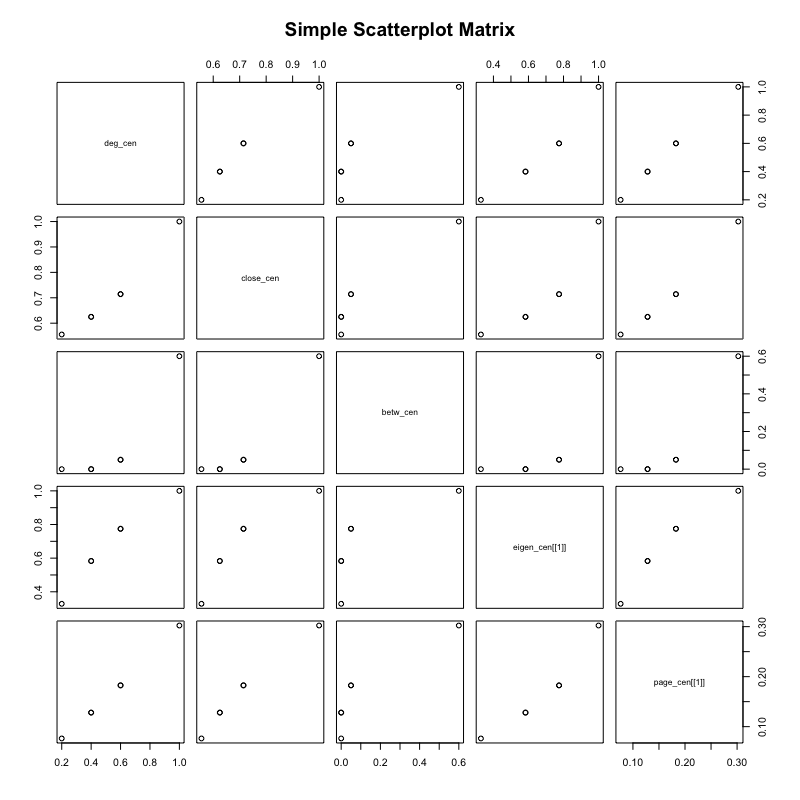
\includegraphics[scale=0.5]{Fig1.png}
\end{figure}

\begin{figure}[ht!]
	\centering
	\captionof{figure}{Scatter plot} \label{tab:figure}
	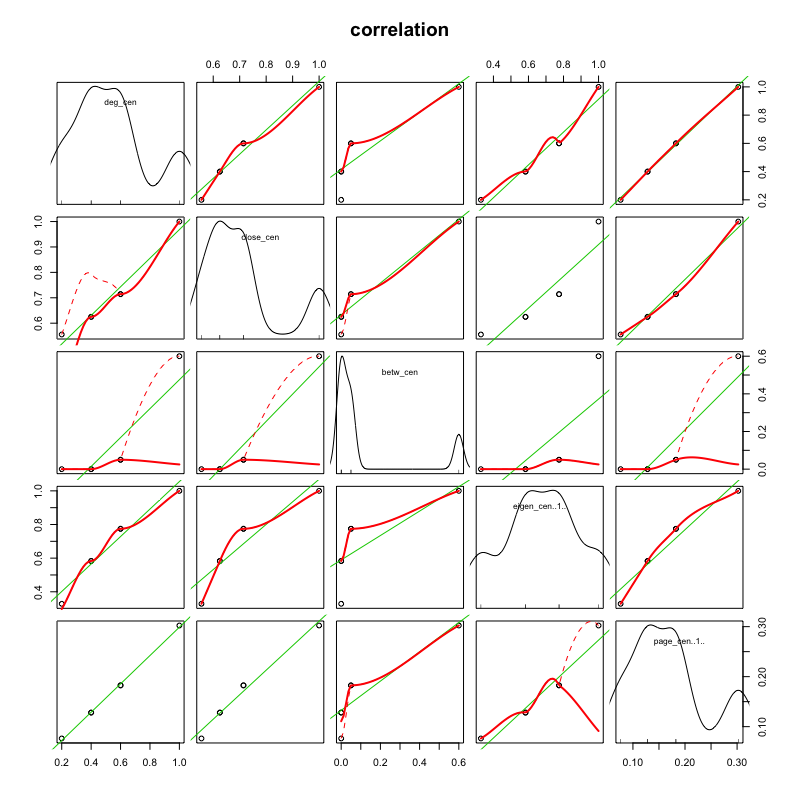
\includegraphics[scale=0.5]{Fig2.png}
\end{figure}




\end{document}	